% !TEX program = xelatex
% ============================================================
%  2026 年度“策联杯”数学建模精英联赛 —— 论文模板
%  编译方式：XeLaTeX（务必使用 XeLaTeX，而非 pdfLaTeX）
%  使用说明：见同目录《论文编写与修改参考.md》
%
%  标题层级约定：
%    一级标题：论文题目
%    二级标题：摘要 / 一、问题重述 / 二、问题分析 / 三、模型假设
%              / 四、符号说明 / 五、模型的建立与求解 / 六、结论
%              / 参考文献 / 附录（后两者按惯例不编号）
%    三级标题：1.1、1.2、2.1……
% ============================================================
\documentclass[UTF8,zihao=-4]{ctexart}

% ---------------- 页面设置 ----------------
\usepackage[top=2.5cm,bottom=2.5cm,left=2.5cm,right=2.5cm]{geometry}

% 页眉页脚：取消所有页眉，仅保留页脚中部页码（plain 样式：无页眉、页脚居中）
\pagestyle{plain}

% ---------------- 数学公式 ----------------
\usepackage{amsmath,amssymb,amsthm}

% ---------------- 图表与代码 ----------------
\usepackage{graphicx}
\usepackage{booktabs}   % 三线表
\usepackage{longtable}  % 长表格（可跨页，用于符号说明等超一页的表格）
\usepackage{multirow}
\usepackage{array}
\usepackage{float}      % 用 [H] 精确控制图表位置
\usepackage{caption}
\usepackage{listings}   % 附录中贴源代码用
\usepackage{xcolor}

% ---------------- 图表标题格式（按需调整） ----------------
\captionsetup{font=small,labelfont=bf}

% ---------------- 代码样式（附录贴源代码用，按需调整） ----------------
\lstset{
  basicstyle=\small\ttfamily,
  numbers=left,
  numberstyle=\tiny,
  frame=single,
  breaklines=true,
  keywordstyle=\color{blue},
  commentstyle=\color{gray},
  stringstyle=\color{red!70!black},
  showstringspaces=false,
}

% ---------------- 标题与序号设置 ----------------
% 二级标题编号：一、二、三……（摘要、参考文献、附录不编号）
% 三级标题编号：1.1、1.2、2.1……（阿拉伯数字，带上级序号）
% 一级标题（论文题目）与二级标题（各节标题）均居中
\ctexset{
  section = {
    format    = {\zihao{3}\bfseries\centering},
    number    = \chinese{section},
    name      = {,、},          % 编号后加“、”，如“一、”
    aftername = {},
  },
  subsection = {
    format    = {\zihao{4}\bfseries},
    number    = \arabic{section}.\arabic{subsection},
    aftername = {\quad},        % 编号与标题之间空一格
  },
  subsubsection = {
    format    = {\zihao{-4}\bfseries},
    number    = \arabic{section}.\arabic{subsection}.\arabic{subsubsection},
    aftername = {\quad},
  },
}

% 正文引用处用 \cite{标签} 标注，文献条目在文末 \begin{thebibliography} 中给出
\newcommand{\upcite}[1]{\textsuperscript{\cite{#1}}}

% 图表编号：按二级标题（节）编号，如“图5.1”“表2.1”，每节重新从 1 计数
\numberwithin{figure}{section}
\numberwithin{table}{section}
\renewcommand{\thefigure}{\arabic{section}.\arabic{figure}}
\renewcommand{\thetable}{\arabic{section}.\arabic{table}}

\begin{document}

% ============================================================
%  论文题目（一级标题）
%  注意：任何地方都不得出现参赛队号、姓名、学校等信息
% ============================================================
\begin{center}
  {\zihao{2}\bfseries 论文题目}
\end{center}

% ============================================================
%  摘要（二级标题，不编号；位于第一页，含标题与关键词，不超过一页）
%  （暂不撰写，待正文完成后补充）
% ============================================================
\section*{摘要}

（摘要暂缓撰写，待正文完成后补充。）

\vspace{1em}
\noindent\textbf{关键词：}关键词1；关键词2；关键词3；关键词4

% 摘要页结束，正文从第二页开始
\clearpage

% ============================================================
%  正文（从第二页开始，整体控制在 30 页以内，不要目录）
% ============================================================

% ---------------- 一、问题重述 ----------------
\section{问题重述}

\subsection{问题背景}

海上油田通常由多个油气田及配套生产设施共同构成，各类海上设施相互协作，承担油气开采、处理外输、设备检维修以及人员生活保障等任务。由于海上油气生产具有连续作业的特点，生产运行、安全管理、设备维修和后勤保障等环节均需要不同专业人员长期驻守，共同保障海上油田安全、稳定运行。

海岗员工通常在设施上连续工作和生活一段时间，到期后集中换班。倒班时，接班人员出海、离岗人员返回陆地；生产任务和检维修安排的变化还会带来不同海上设施之间的人员穿梭。人员往返主要由直升机运输，海上设施通常设有直升机停机坪。人员运输任务按业务性质分为应急处置、增储上产、常规倒班和临时任务四类，实际运行中的业务保障次序通常按这一顺序；其中，将人员从陆地机场前往海上设施称为出海，从海上设施返回陆地机场称为海返，从一座海上设施前往另一座海上设施称为穿梭。

本题聚焦海上油田的人员运输，包括 3 座陆地机场（A01、A02、A03）和 52 座海上设施（F001 至 F052），其中有 8 座海上设施设有加油站（F006、F011、F018、F024、F031、F038、F044、F050），可为直升机补充燃油。直升机的可用机型为 T1、T2、T3 三种，主要参数见表~\ref{tab:aircraft}。每个架次从机场满油起飞，到达每一处地点（含最终返回机场）时的剩余燃油不得低于该机型的最低安全余油量；在可加油设施停靠时可选择是否加油（加油即加满），不加油时每次停靠至少 10 分钟、加油时至少 20 分钟。本题的主要考核目标为飞机使用时间，人员总在途时间与座位利用率也是需要考虑的重要因素。

\subsection{问题提出}

题目共提供四个数据文件和三个问题的结果模板，要求完成以下三个问题：

\textbf{问题一（单向出海运输）}：\texttt{peopleQ1.csv} 给出 1600 条出海需求，请为这些需求编排运载计划。本问不考虑最早可登机时间、最晚需到达时间和业务性质优先级的约束，假设有足够多的飞机可用，在最小化总飞机使用时间的基础上尽可能优化其他因素（如座位利用率、油耗）。结果需呈现在 \texttt{q1-assignments.csv} 和 \texttt{q1-routes.csv} 中，并在论文中给出总飞机使用时间、人员总在途时间、总架次数、总燃油消耗量以及座位利用率五项指标。

\textbf{问题二（出海、海返与穿梭联合运输）}：\texttt{peopleQ2.csv} 给出 4000 条包括出海、海返和穿梭的需求，请为这些需求编排运载计划。与问题一相同，本问不考虑最早可登机时间、最晚需到达时间和业务性质优先级的约束，假设有足够多的飞机可用，在最小化总飞机使用时间的基础上尽可能优化其他因素。结果需呈现在 \texttt{q2-assignments.csv} 和 \texttt{q2-routes.csv} 中，并给出与问题一相同的五项指标。

\textbf{问题三（带时间要求的多日排班）}：\texttt{peopleQ3.csv} 在问题二的基础上增加了最早离开起点时刻、最晚送达时刻和业务性质，需求时间在 2026-08-03 00:00 至 2026-08-10 00:00 之间。本问考虑飞机数量限制，使用 24 架飞机，每架飞机在规划开始时停放在所属机场；机场运营时段内，飞机可在 06:00 至 18:00 之间起飞，且不晚于 20:00 返回机场，飞机不得在海上设施过夜，完成一个架次后至少经过 30 分钟的机场周转。在四类任务中，临时任务有可能为减少运输开销而被取消：请先在不考虑临时任务的情况下编排计划，得到其总飞机使用时间，再在不超过该总时间的条件下将临时人员加入，尽可能多地满足其运输需求。结果需呈现在 \texttt{q3-assignments.csv} 和 \texttt{q3-routes.csv} 中，并给出临时人员满足情况及五项指标。

\begin{table}[H]
  \centering
  \caption{三种直升机的主要参数}
  \label{tab:aircraft}
  \begin{tabular}{lccccc}
    \toprule
    机型 & 座位数 & 速度（km/h） & 油耗（kg/km） & 油箱容量（kg） & 最低安全余油量（kg） \\
    \midrule
    T1 & 12 & 250 & 3.4 & 1000 & 150 \\
    T2 & 16 & 220 & 2.5 & 1150 & 150 \\
    T3 & 19 & 190 & 2.9 & 1600 & 200 \\
    \bottomrule
  \end{tabular}
\end{table}

% ---------------- 二、问题分析 ----------------
\section{问题分析}

\subsection{问题一}\label{sec:analysis}

问题一可抽象为一个\textbf{多机场、多机型、带容量与燃油约束的单向车辆路径问题}（经典 CVRP 的变体）。与经典 VRP 相比，其差异主要体现在：

\begin{enumerate}
  \item \textbf{单向运送}：架次只执行“机场 $\to$ 若干海上设施 $\to$ 原机场”的环游，人员只下不上（出海方向），无需考虑返程载客；
  \item \textbf{人员不可换乘}：每名人员必须由同一架次从其起点直接送到终点，中途不得换机；
  \item \textbf{多机型}：T1/T2/T3 的座位数、速度、油耗、航程均不同，机型是决策变量而非固定参数；
  \item \textbf{燃油约束}：满油起飞、全程剩余油量不低于最低安全余油量，可在 8 个可加油设施中途加油（加满）；
  \item \textbf{停靠次数上限}：每架次最多 5 次海上着陆（加油停靠也计入着陆次数）。
\end{enumerate}

\textbf{目标函数的本质}。一个架次的总使用时间由飞行时间与停靠时间构成：
\begin{equation}
  T_r = \frac{d_r^{\mathrm{TSP}}}{v_{m_r}} + 10\,|S_r| + 10\,g_r,
\end{equation}
其中 $d_r^{\mathrm{TSP}}$ 为该架次的环游飞行距离（由访问顺序决定），$v_{m_r}$ 为机型速度，$|S_r|$ 为海上停靠次数（每次 10 分钟），$g_r$ 为其中加油的停靠次数（加油停靠每次 20 分钟，比普通停靠多 10 分钟）。由于设施间平均距离（约 180 km）\textbf{小于}机场到设施的平均距离（约 254 km），把地理相邻的设施合并进同一架次能省去多次“机场往返”，这正是优化空间所在；而合并受到座位数（$\le 19$）与停靠次数（$\le 5$）的双重约束。因此问题一的本质是：\textbf{在容量与航程约束下，对设施进行聚类分组，每组一个架次做 TSP 环游并选机型，使总时间最小}。

\textbf{数据特征}。对 \texttt{peopleQ1.csv} 与 \texttt{distances.csv} 分析得到如下结论（表~\ref{tab:demand}、图~\ref{fig:q1_od}）：1600 条需求中，指定机场的 247 人按“三块”分布（A01$\to$F001$\sim$F017、A02$\to$F018$\sim$F035、A03$\to$F036$\sim$F052），起点为 LAND 的 1353 人则均匀覆盖全部 52 个设施；52 个设施全部有需求，每设施 19$\sim$51 人、均值 30.8 人。三种机型的最大不加油航程差异显著（表~\ref{tab:range}），T1 航程最短（250 km）、仅能单程覆盖部分设施，T3 航程最长（约 483 km）但速度最慢，远端设施往返仍须中途加油，故\textbf{燃油是硬约束}，加油点的选择与插入是航线可行性的必要条件。

\begin{table}[H]
  \centering
  \caption{问题一需求分布统计}
  \label{tab:demand}
  \begin{tabular}{ll}
    \toprule
    项目 & 结论 \\
    \midrule
    需求规模 & 1600 人（指定机场 247 人 + LAND 1353 人） \\
    设施需求 & 52 个设施全部有需求，每设施 19$\sim$51 人，均值 30.8 \\
    机场自然分块 & F001$\sim$F017$\to$A01、F018$\sim$F035$\to$A02、F036$\sim$F052$\to$A03，负载 499/598/503 \\
    纯就近分配 & A01=944、A02=275、A03=381（严重失衡） \\
    \bottomrule
  \end{tabular}
\end{table}

\begin{figure}[H]
  \centering
  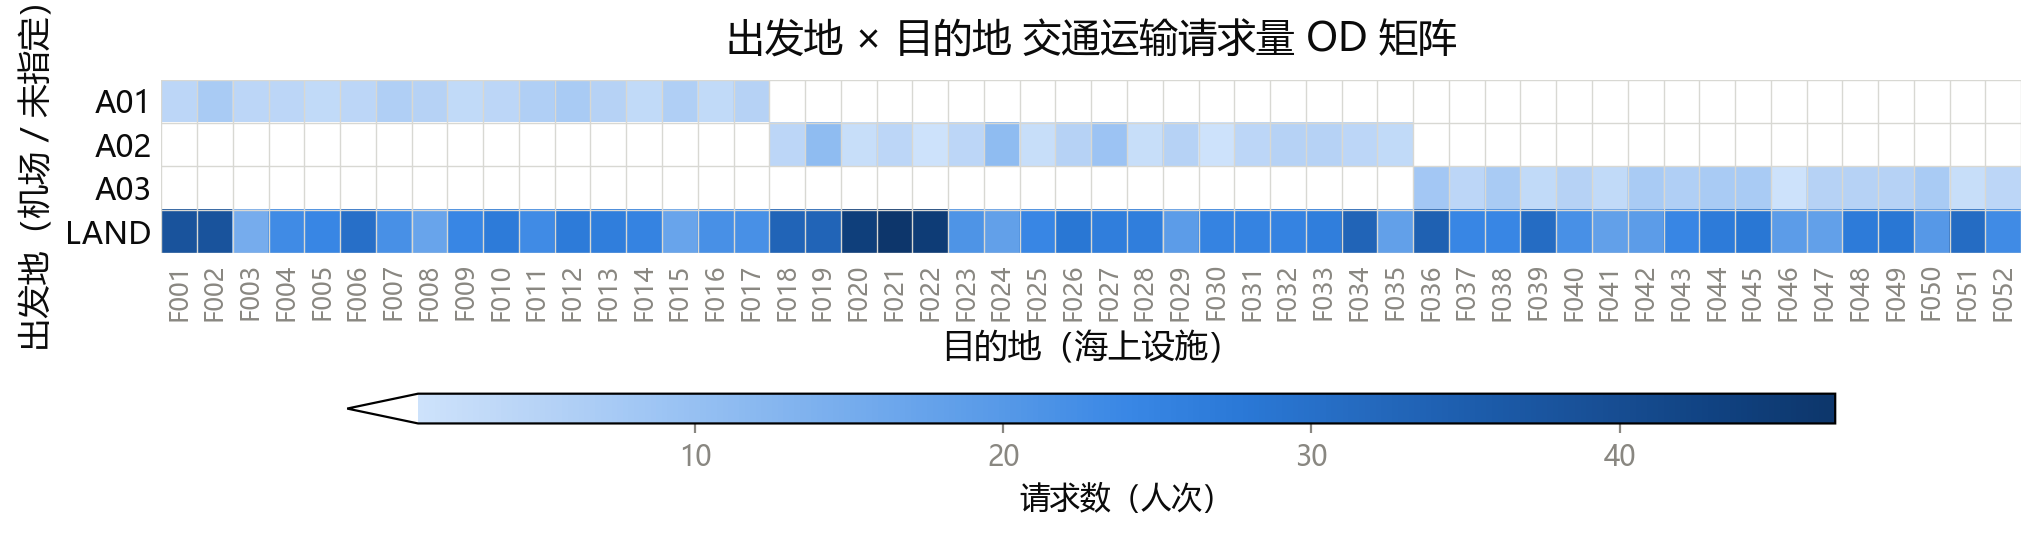
\includegraphics[width=\linewidth]{../output/question1_OD矩阵热力图.png}
  \caption{1600 条出海需求按“出发地 $\times$ 目的地”聚合的 OD 矩阵热力图}
  \label{fig:q1_od}
\end{figure}

\begin{table}[H]
  \centering
  \caption{三种机型续航能力对比（可用燃油 $=$ 油箱容量 $-$ 最低安全余油量，最大不加油航程 $=$ 可用燃油 $\div$ 油耗）}
  \label{tab:range}
  \begin{tabular}{lccccccc}
    \toprule
    机型 & 座位数 & 速度(km/h) & 油耗(kg/km) & 油箱容量(kg) & 最低余油(kg) & 可用燃油(kg) & 最大不加油航程(km) \\
    \midrule
    T1 & 12 & 250 & 3.4 & 1000 & 150 & 850 & 250 \\
    T2 & 16 & 220 & 2.5 & 1150 & 150 & 1000 & 400 \\
    T3 & 19 & 190 & 2.9 & 1600 & 200 & 1400 & $\approx$483 \\
    \bottomrule
  \end{tabular}
\end{table}

\subsection{问题二}

问题二在问题一单向出海的基础上，进一步引入海返（海上设施返回陆地）与穿梭（海上设施之间）两类需求，共 4000 条。其本质升级为\textbf{带同时取送的车辆路径问题（VRPSPD）}：同一架次既承载出海的到达、又承载海返的出发，机上人数沿环游先降后升、不再单调。与问题一相比有三点本质差异：

\begin{enumerate}
  \item \textbf{人员是 OD 对而非“送到即可”}：每名人员必须由同一架次从其起点直送终点，中途不得换乘；
  \item \textbf{载荷剖面非单调}：设施上既有下机（出海、穿梭到达）又有上机（海返、穿梭出发），机上人数先降后升或反复波动；
  \item \textbf{环游有向}：穿梭 $i\to j$ 要求 $i$ 在 $j$ 之前被访问，环游方向成为决策的一部分，正反两向是不同的候选架次。
\end{enumerate}

\textbf{数据特征}。对 \texttt{peopleQ2.csv} 与 \texttt{distances.csv} 逐设施统计，得到三点结论（图~\ref{fig:q2_od}），它们是本问建模与求解的基石：

\begin{enumerate}
  \item \textbf{出海与海返总量平衡}：各 1600 条，且出海即问题一 \texttt{peopleQ1} 的子集；
  \item \textbf{逐设施近乎配对}：设施 $d$ 的净差 $q_d^{\mathrm{out}}-q_d^{\mathrm{ret}}$ 落在 $[-4,+6]$，其中 48/52 个设施在 $\pm3$ 以内，即“送去多少人、几乎接回多少人”；
  \item \textbf{穿梭全部同区块短途}：56 个穿梭 OD 的起终点都落在同一区块（F001$\sim$F017 / F018$\sim$F035 / F036$\sim$F052），不跨机场，每个 OD 仅 9$\sim$19 人。
\end{enumerate}

由结论 (1)(2)，出海与海返可组织为\textbf{往返环游}，载荷近似恒定，在容量上退化为问题一；穿梭才是本问真正新增的运力要素，规模小、短途、同区块，可在环游途中顺路承载。

\begin{figure}[H]
  \centering
  % 待补充：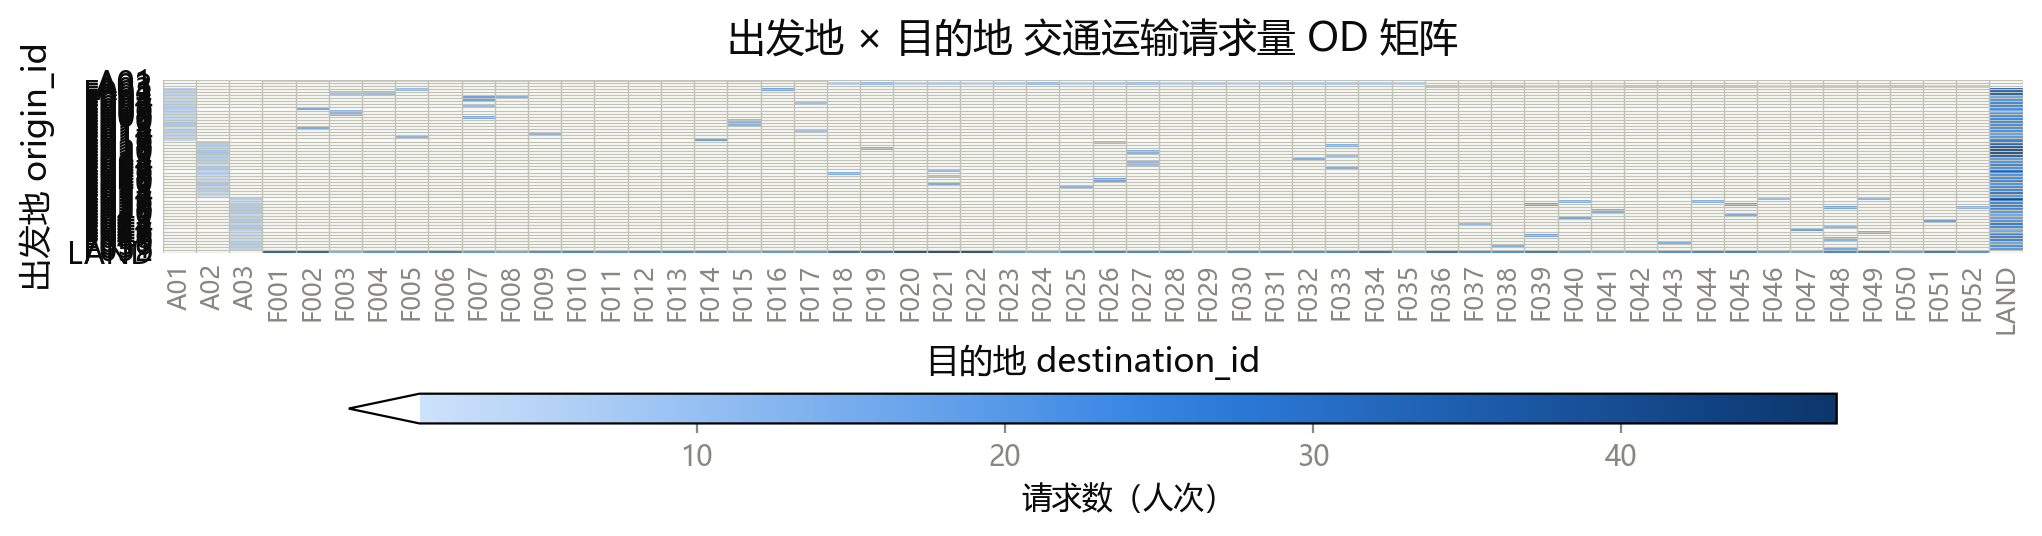
\includegraphics[width=\linewidth]{../output/question2_OD矩阵热力图.png}
  \fbox{\parbox{0.85\linewidth}{\centering 图占位：问题二 OD 矩阵热力图（待补充） \\[2.5cm]}}
  \caption{4000 条出海、海返与穿梭需求按 OD 聚合的热力图}
  \label{fig:q2_od}
\end{figure}

\subsection{问题三}
（问题三的建模与分析待后续完成。）

% ---------------- 三、模型假设 ----------------
\section{模型假设}

结合题目给定条件与实际场景，作如下合理假设：

\begin{enumerate}
  \item 人员上下机、地面调度时间忽略不计（题目未给出）；
  \item 飞行速度与单位距离油耗不随载客量变化（题目给定）；
  \item 忽略机场、设施、加油站的并发容量限制（题目给定）；
  \item 停靠时间取最小：不加油 10 分钟、加油 20 分钟，时间向上取整到整数分钟；
  \item 距离矩阵对称且满足三角不等式（实际地理距离，可直接用于 TSP 环游）；
  \item 针对问题一与问题二，假设飞机数量充足，且不考虑最早可登机时间、最晚需到达时间与业务性质优先级（题目给定）。
\end{enumerate}

% ---------------- 四、符号说明 ----------------
\section{符号说明}

\begin{longtable}{p{3.4cm}@{\qquad}p{10.2cm}}
  \caption{主要符号说明}\label{tab:symbols}\\
  \toprule
  符号 & 含义 \\
  \midrule
  \endfirsthead
  \toprule
  符号 & 含义 \\
  \midrule
  \endhead
  $\mathcal{A}=\{A01,A02,A03\}$ & 陆地机场集合 \\
  $\mathcal{F}=\{F001,\dots,F052\}$ & 海上设施集合，$|\mathcal{F}|=52$ \\
  $\mathcal{R}\subset\mathcal{F}$ & 可加油设施集合（共 8 个） \\
  $\mathcal{M}=\{T1,T2,T3\}$ & 直升机机型集合 \\
  \midrule
  $c_m,\ v_m,\ f_m,\ U_m,\ \underline{u}_m$ & 机型 $m$ 的座位数、速度(km/h)、油耗(kg/km)、油箱容量(kg)、最低安全余油量(kg) \\
  $\bar{d}_m=\dfrac{U_m-\underline{u}_m}{f_m}$ & 机型 $m$ 的最大不加油航程(km) \\
  $d_{uv}$ & 节点 $u,v\in\mathcal{A}\cup\mathcal{F}$ 间的距离(km)，对称 \\
  $q_d$ & 设施 $d$ 的出海总人数（指定机场 + LAND 合计） \\
  $\sigma(d)\in\mathcal{A}$ & 设施 $d$ 的归属机场（按编号分块） \\
  $\mathcal{F}_a=\{d:\sigma(d)=a\}$ & 机场 $a$ 服务的设施集合（分块后固定） \\
  $D_d$ & 设施 $d$ 的候选拆分方案集合 \\
  $n_s,\ p_s$ & 拆分方案 $s$ 的满座架次数、尾数份人数 \\
  \midrule
  $y_s\in\{0,1\}$ & 是否选取设施 $d$ 的拆分方案 $s$ \\
  $\lambda_r\in\mathbb{Z}_+$ & 尾数合并架次 $r$ 的使用次数 \\
  \midrule
  $S_r\subset\mathcal{F}$ & 架次 $r$ 访问的设施集合，$|S_r|\le 5$ \\
  $g_r$ & 架次 $r$ 的加油停靠次数（$0\le g_r\le |S_r|$） \\
  $d_r^{\mathrm{TSP}}$ & 架次 $r$ 的环游飞行距离(km) \\
  $T_r$ & 架次 $r$ 的总飞机使用时间(min) \\
  \midrule
  $z_{LP},\ z_{IP}$ & 集合划分模型的 LP 松弛下界、整数最优值(min) \\
  $\eta$ & 座位利用率 \\
  \midrule
  $q_d^{\mathrm{out}},\ q_d^{\mathrm{ret}}$ & 设施 $d$ 的出海、海返总人数（问题二） \\
  $q^{\mathrm{sh}}_{(i,j)}$ & 穿梭 OD 对 $(i,j)$ 的需求人数（问题二） \\
  $(d_c,p_c)$ & 设施 $d$ 在机型 $c$ 下的成对尾数（出海尾数、海返尾数） \\
  $h_{(i,j)}$ & 某架次承载的穿梭 OD $(i,j)$ 尾数 \\
  $n_{r,(i,j)}$ & 架次 $r$ 承载 OD 对 $(i,j)$ 的人数 \\
  $D_{(i,j)}$ & OD 对 $(i,j)$ 的需求总人数 \\
  $\pi_{(i,j)}$ & 主问题 OD 覆盖约束的对偶价 \\
  $L_t$ & 第 $t$ 站后弧段上的机上人数（载荷剖面） \\
  \bottomrule
\end{longtable}

% ---------------- 五、模型的建立与求解 ----------------
\section{模型的建立与求解}

\subsection{问题一}

\subsubsection{建模总体思路与问题分解}

问题一要求最小化总飞机使用时间，整体上是一个多机场、多机型、带容量与燃油约束的单向 VRP：需同时决定每名乘客的起飞机场、每架次访问的设施集合与顺序、机型以及加油方案，规模大且 NP-hard，直接整体求解不可行。为此，建模的第一步是寻找\textbf{可分性}，把大问题化为可精确求解的小问题。

可分性来自三条结构性事实：\textbf{(1) 人员不可换乘}——每名人员由同一架次从起点直送终点，架次之间无乘客衔接；\textbf{(2) 架次不跨机场中转}——任一架次从某机场起飞、最终返回同一机场，全程只服务该机场周边的设施；\textbf{(3) 飞机数量充足}——机场之间不存在机队争夺。由事实 (1)(2)，任一架次自始至终只服务于其起飞机场周边的设施，不同机场的架次互不牵扯；由事实 (3)，机场间无需共享资源。故\textbf{只要每名乘客的起飞机场被确定，整体问题即退化为三个互不相干、结构完全相同的单机场子问题}：
\begin{equation}
  \min \sum_{a\in\mathcal{A}} \mathrm{VSP}(a),
\end{equation}
其中 $\mathrm{VSP}(a)$ 为机场 $a$ 的单机场航线编排子问题。

唯一障碍是 1353 名 LAND 乘客没有指定起飞机场：若把机场选择留作决策变量，三个机场将通过 LAND 乘客相互耦合，整体性无法破除。下一节借助“设施沿海岸线线性排列、编号与机场位置一致”的地理结构，把 LAND 乘客按设施分块固定归属机场，从而将机场选择从决策变量退化为固定参数，完成分解。

\subsubsection{需求分块固定分配}

设施编号 F001$\sim$F052 沿海岸线自北向南线性排列，与三个机场的位置分布一致，故按编号等分为三段即可同时兼顾“就近”与“均衡”：
\begin{equation}
  \sigma(d)=
  \begin{cases}
    A01, & d\in\{\text{F001},\dots,\text{F017}\}\\
    A02, & d\in\{\text{F018},\dots,\text{F035}\}\\
    A03, & d\in\{\text{F036},\dots,\text{F052}\}
  \end{cases}
\end{equation}
三段负载分别为 499/598/503 人，接近均衡；且编号顺序与海岸线走向一致，各段设施就近其对应机场（见图~\ref{fig:q1_demand}）。将设施 $d$ 的全部需求统一由 $\sigma(d)$ 服务，则各机场的设施集合与人数均为固定参数：
\begin{equation}
  \mathcal{F}_a=\{d:\sigma(d)=a\},\qquad
  q_{d,a}=\begin{cases}q_d, & \sigma(d)=a\\[2pt] 0, & \text{否则}\end{cases}
\end{equation}
这一步的实质是把 LAND 的机场选择从决策变量退化为固定参数，模型无需再对 1353 名 LAND 乘客逐一建立“去哪座机场”的约束，子问题规模大幅下降。

\begin{figure}[H]
  \centering
  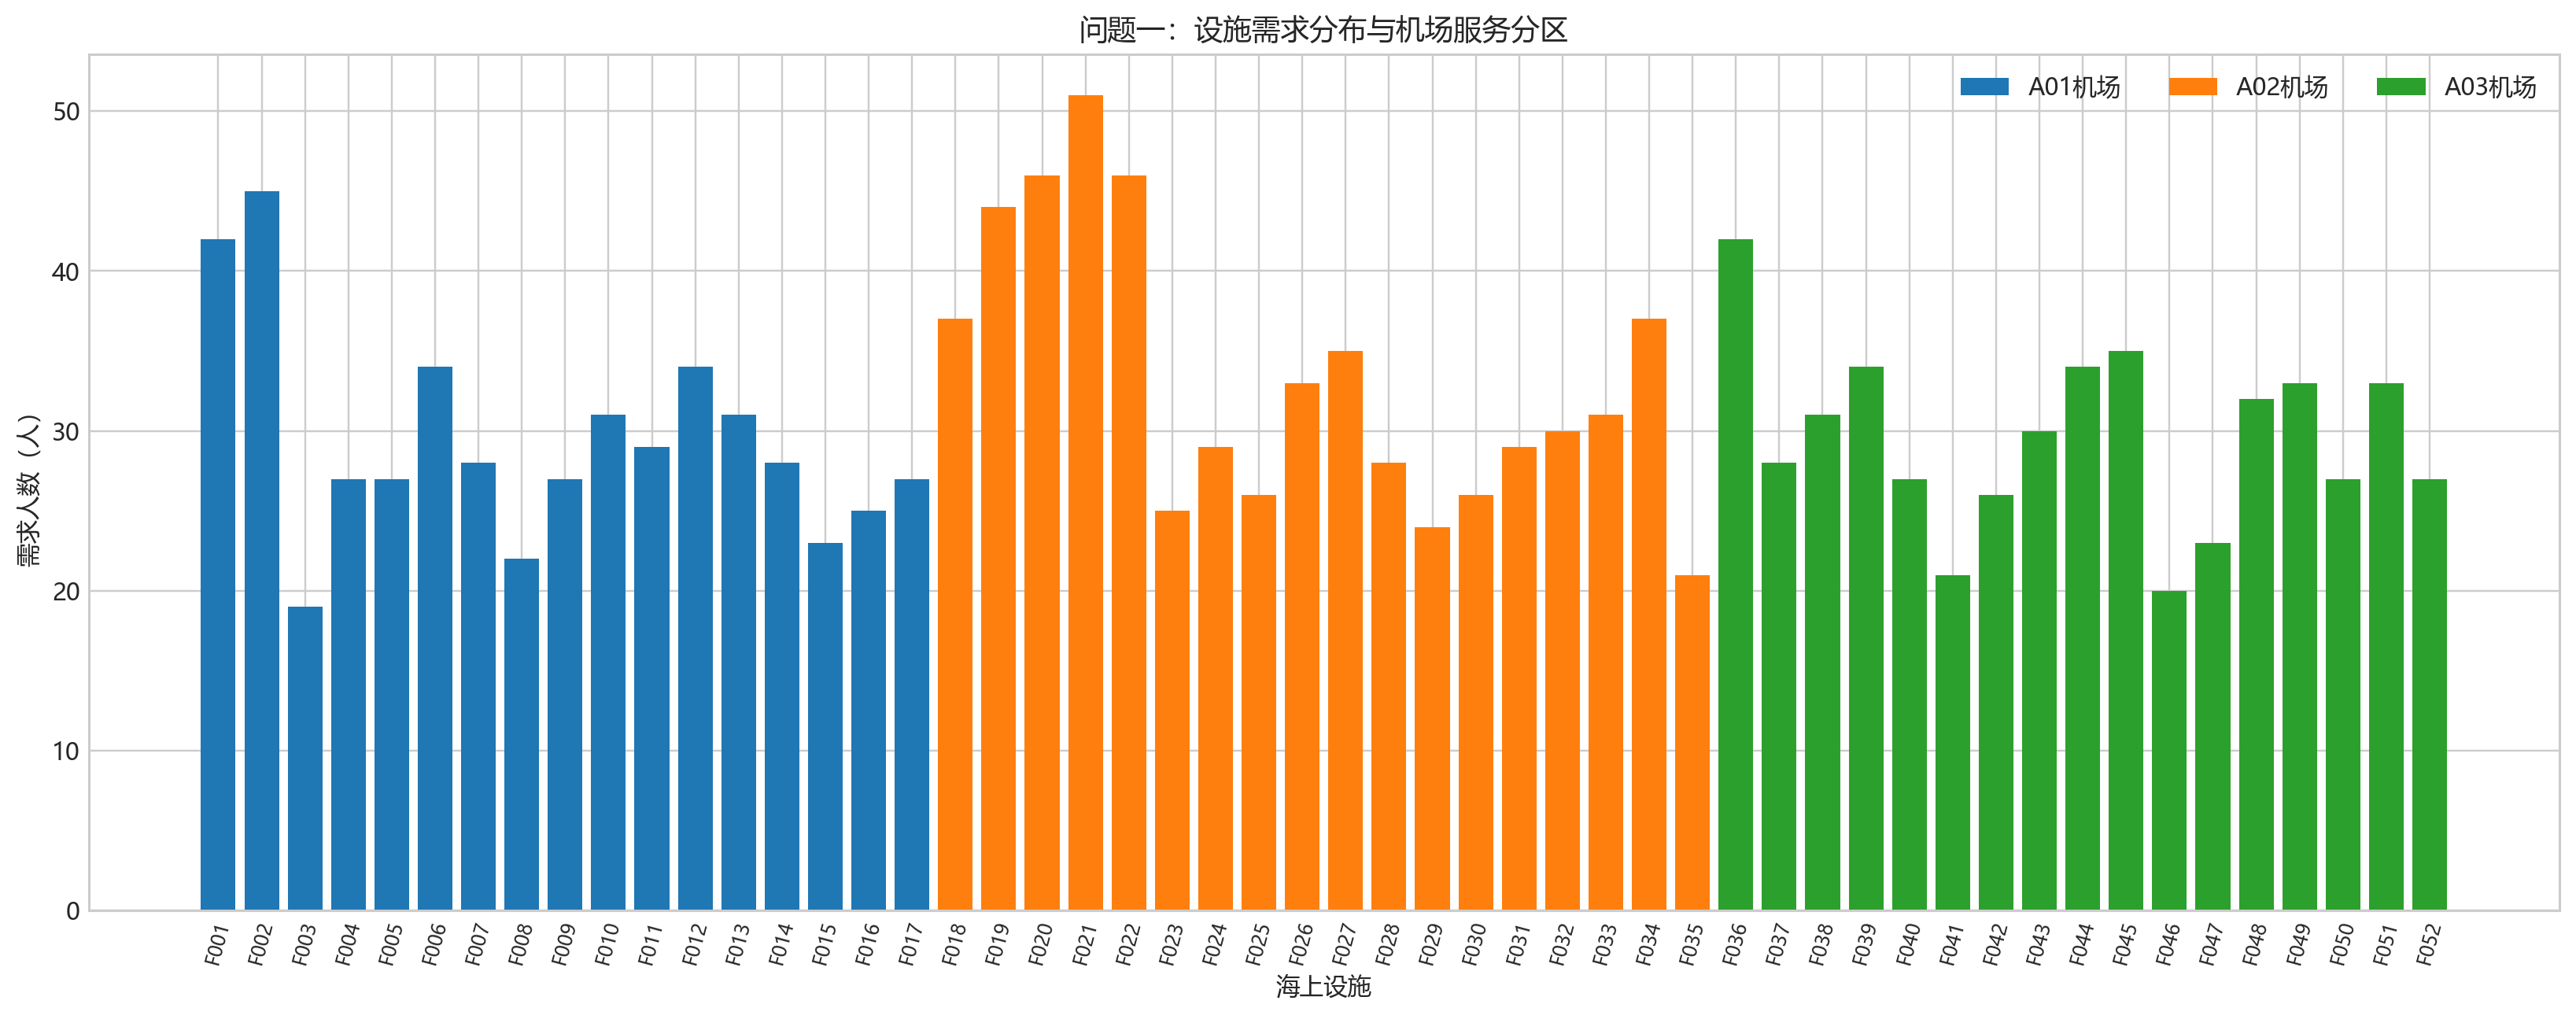
\includegraphics[width=0.9\linewidth]{../output/问题一_设施需求分布图.png}
  \caption{52 个海上设施的出海需求分布及其机场分块归属}
  \label{fig:q1_demand}
\end{figure}

\subsubsection{机型感知拆分与满座架次}

固定一个机场 $a$，其设施集合 $\mathcal{F}_a$ 与人数 $q_d$ 均为已知参数。由于单机最多 19 座而每设施需求 19$\sim$51 人，任一设施都须由多架次共同运送（split delivery）。对设施 $d$ 的每种机型 $m$ 生成一个候选拆分方案 $s=(m_s,n_s,p_s)$：
\begin{equation}
  n_s=\left\lfloor \frac{q_d}{c_{m_s}}\right\rfloor,\qquad p_s=q_d-c_{m_s}\,n_s,
\end{equation}
其中 $c_{m_s}$ 为方案 $s$ 的机型座位数（T1$\leftrightarrow$12、T2$\leftrightarrow$16、T3$\leftrightarrow$19），$n_s$ 为满座架次数，$p_s$ 为拆不尽的尾数份人数（$0\le p_s<c_{m_s}$）。例如 $q_d=29$：T3 得 $(19,1,10)$、T2 得 $(16,1,13)$、T1 得 $(12,2,5)$，三种方案构成候选集合 $D_d$，由后续整数规划统一择优。

满座份人数恰等于座位数，满载单飞已是该部分人员的最快运送方式——再并入其他设施只会增加飞行距离与停靠次数，绝无收益。故满座架次不参与合并，直接固化为固定成本：
\begin{equation}
  T^{\text{满}}(d,m)=\frac{2\,d_{\sigma(d),d}}{v_m}+10+10\,g,
\end{equation}
即机场 $\sigma(d)$ 到该设施往返的飞行时间加一次停靠（10 分钟）；$g\in\{0,1\}$ 表示该满座架次是否在可加油设施加油（加油停靠按 20 分钟计），由燃油判据确定。每个满座架次独立往返，$n_s$ 个满座架次共贡献 $n_s\,T^{\text{满}}(d,m_s)$，从优化变量中消去。

\subsubsection{尾数合并架次与集合划分整数规划}

真正需要决策的只剩各设施的尾数份。以 $(d,m_s)$ 标识一条尾数份（设施 $d$ 在机型 $m_s$ 下的尾数，人数 $p_s$），一个架次可把若干条来自不同设施的尾数份合并为一条“机场$\to$若干设施$\to$机场”的环游，一次飞多个设施以省去多次机场往返。设尾数合并架次 $r$ 含尾数份集合 $\Theta_r$、访问设施集合 $S_r$、机型 $m_r$，须满足容量与停靠次数约束：
\begin{equation}
  \sum_{(d,m_s)\in\Theta_r} p_s \le c_{m_r},\qquad |S_r|\le 5,
\end{equation}
且同一设施至多出现一条尾数份（每个设施最终只选一个拆分方案）。其成本为环游飞行时间加停靠时间：
\begin{equation}
  T_r=\frac{d_r^{\mathrm{TSP}}}{v_{m_r}}+10\,|S_r|+10\,g_r.
\end{equation}

在此基础上建立集合划分整数规划：为每个拆分方案设 0-1 变量 $y_s$，为每条尾数合并架次设整数变量 $\lambda_r$，得
\begin{equation}
  \min \sum_{d}\sum_{s\in D_d} y_s\,n_s\,T^{\text{满}}(d,m_s)+\sum_{r}T_r\,\lambda_r,\label{eq:obj}
\end{equation}
\begin{equation}
  \text{s.t.}\quad \sum_{s\in D_d} y_s=1,\quad \forall d\in\mathcal{F}_a,\label{eq:part}
\end{equation}
\begin{equation}
  \sum_{r:\ (d,m_s)\in\Theta_r}\lambda_r = y_s,\quad \forall d,\ \forall s\in D_d,\ p_s>0,\label{eq:align}
\end{equation}
\begin{equation}
  y_s\in\{0,1\},\qquad \lambda_r\in\mathbb{Z}_+.\label{eq:lambda}
\end{equation}
目标函数第一项为满座架次的固定时间，第二项为尾数合并架次的时间；式~\eqref{eq:part}（每个设施恰选一个拆分方案）保证需求被恰好覆盖，式~\eqref{eq:align} 把所选方案的尾数份与其运载架次对齐；容量与停靠次数上限已内化于架次列 $r$ 的定义，无需显式写出。该模型为纯线性 0-1/整数规划，规模很小，可由求解器直接精确求解。

\subsubsection{燃油可行性约束}

燃油约束是航线的可行性条件而非目标项：在最小化总时间之外，还要求每个架次全程剩余油量不低于安全余油。记架次 $r$ 的路线为 $a=s_0\to s_1\to\cdots\to s_k\to s_{k+1}=a$，飞机满油 $u_0=U_m$ 起飞，到达每站后的剩余油量逐站递推：
\begin{equation}
  u_i=\begin{cases}
    U_m, & s_i\in\mathcal{R}\ \text{且在该站加油}\\
    u_{i-1}-f_m\,d_{s_{i-1},s_i}, & \text{否则},
  \end{cases}\label{eq:fuel}
\end{equation}
可行性要求每一站（含最终返回机场）剩余油量都不低于安全余油：
\begin{equation}
  u_i\ge \underline{u}_m,\quad i=1,\dots,k+1.\label{eq:feasible}
\end{equation}
由于加油即加满，式~\eqref{eq:fuel}--\eqref{eq:feasible} 等价于一条更直观的判据：\textbf{任意两个相邻加油点（含起飞机场与返程机场）之间的累计飞行距离不得超过最大不加油航程 $\bar{d}_m$}。因此燃油检查可简化为“按加油点把路线切成若干段，逐段比较累计距离与 $\bar{d}_m$”。对某段超航程的架次，在其间就近插入 $\mathcal{R}$ 中的加油点即可修复（绕行距离计入 $d_r^{\mathrm{TSP}}$，加油停靠按 20 分钟计并占用停靠次数配额）。

\subsubsection{求解算法}

解耦后每机场仅 17$\sim$18 个设施，即使枚举全部可能的架次，规模仍在可控范围，故采用“\textbf{显式枚举候选 + 集合划分整数规划}”的精确方法，流程如下：

\begin{enumerate}
  \item \textbf{生成拆分候选与满座架次}：对每设施 $d$、每机型 $c\in\{19,16,12\}$，计算 $n_s=\lfloor q_d/c\rfloor$（满座份数）与 $p_s=q_d-c\,n_s$（尾数份人数），满座架次固化为固定成本；
  \item \textbf{枚举尾数合并架次}：筛去 $p=0$ 的尾数份，用深度优先回溯逐份决策“取或不取”，并即时剪枝（累计人数 $>19$、已取个数达 5、或设施重复即不再“取”），得到候选组合 $S$；对每个组合用 $\le 5$ 点的 TSP 求最短环游距离，再对每种容量足够的机型生成一条尾数合并架次列；
  \item \textbf{构建并求解集合划分 IP}：把枚举结果填入式~\eqref{eq:obj}--\eqref{eq:lambda} 的整数规划，用 CBC 求解器精确求解；
  \item \textbf{燃油后置校验与修复}：对每条枚举出的架次，按“相邻加油点间距离 $\le\bar{d}_m$”规则逐列校验，可行的直接保留，超航程的先尝试就近插入加油点修复，仍不可行则弃列；
  \item \textbf{报告 LP 下界与 gap}：将 $y_s,\lambda_r$ 的整性约束放松为连续得到 LP 松弛，其最优值 $z_{LP}$ 构成任何可行排班总时间的下界；记整数最优值为 $z_{IP}$，则 $\text{gap}=\dfrac{z_{IP}-z_{LP}}{z_{LP}}$，gap 越小说明解越接近全局最优。
\end{enumerate}

这种“生成—校验—修复”的流水线把燃油状态排除在整数规划的变量之外，保持 IP 简洁可解。

\subsubsection{求解结果与分析}

用上述模型与算法求解，得到问题一的完整运载计划，核心指标见表~\ref{tab:q1_result}，航线网络见图~\ref{fig:q1_network}，求解结果综合对比见图~\ref{fig:q1_result}。

\begin{table}[H]
  \centering
  \caption{问题一求解结果指标}
  \label{tab:q1_result}
  \begin{tabular}{lc}
    \toprule
    指标 & 数值 \\
    \midrule
    总飞机使用时间 & 15061 min（$\approx$251.02 h） \\
    人员总在途时间 & 131033 min（$\approx$2183.88 h） \\
    总架次数 & 88 \\
    总燃油消耗量 & 120920.1 kg \\
    座位利用率 & 49.68\% \\
    \midrule
    LP 松弛下界 & 15041.00 min \\
    gap & 0.13\% \\
    \bottomrule
  \end{tabular}
\end{table}

\begin{figure}[H]
  \centering
  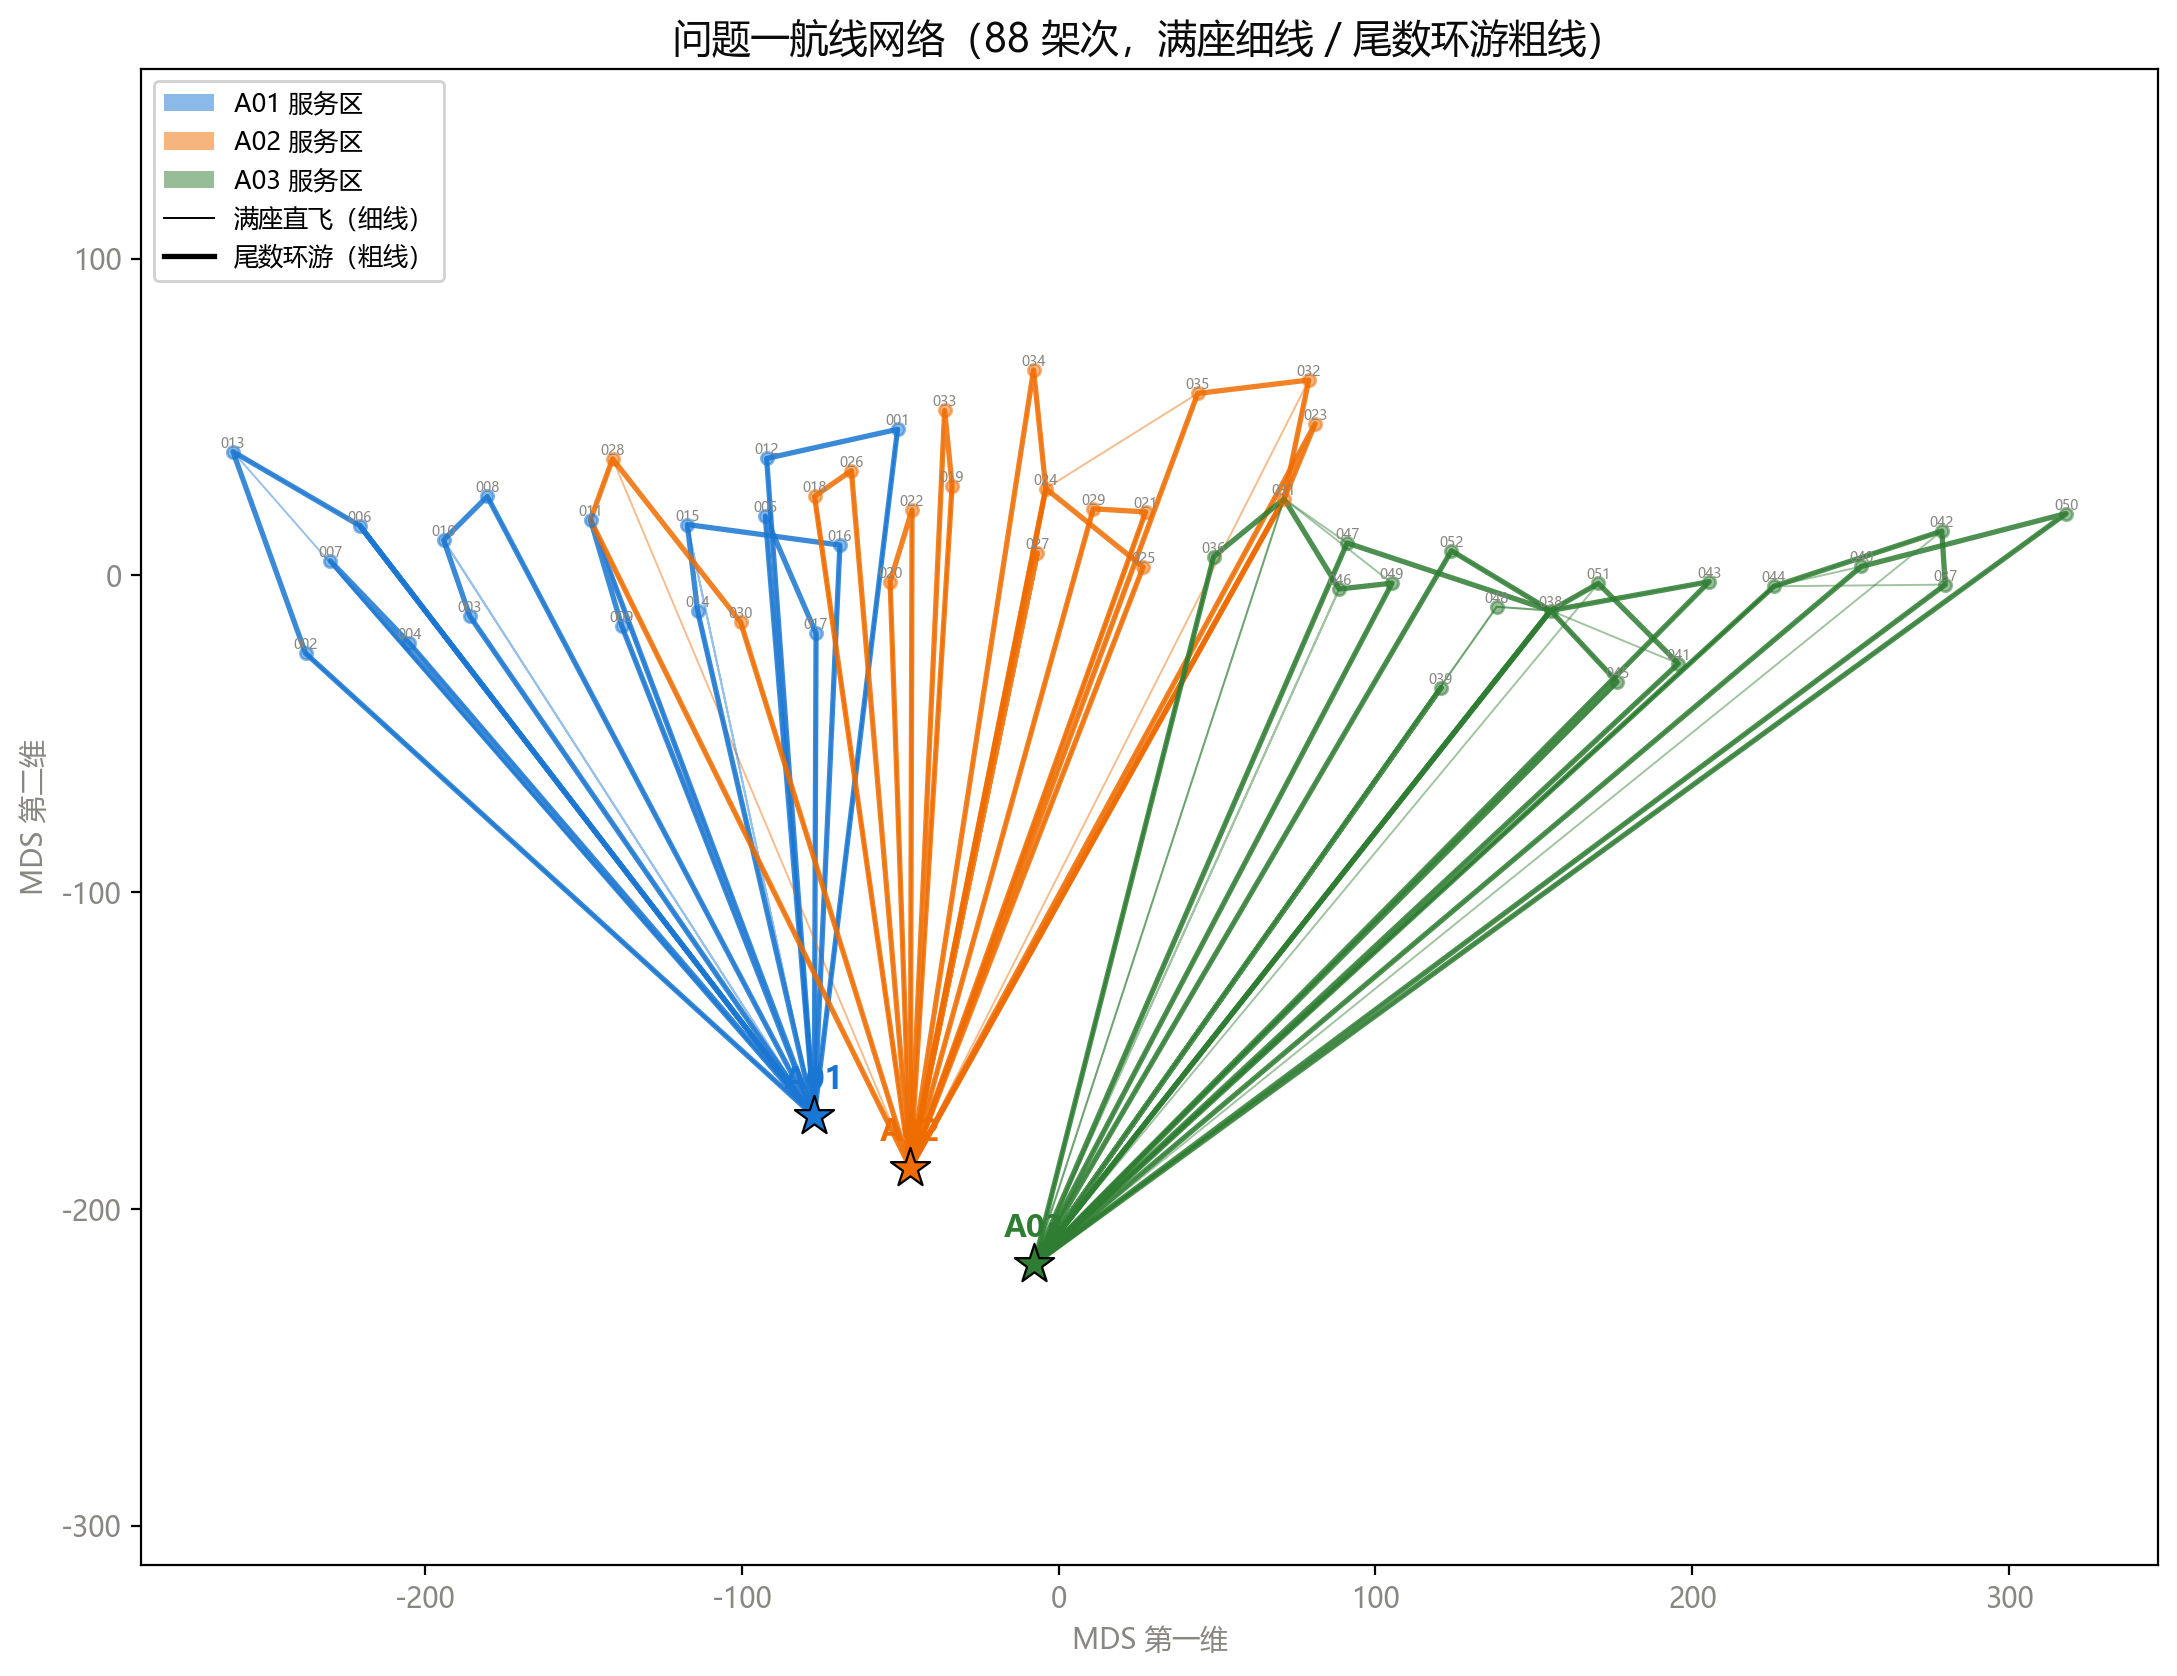
\includegraphics[width=0.95\linewidth]{../output/问题一_航线网络图.png}
  \caption{问题一航线网络图}
  \label{fig:q1_network}
\end{figure}

\begin{figure}[H]
  \centering
  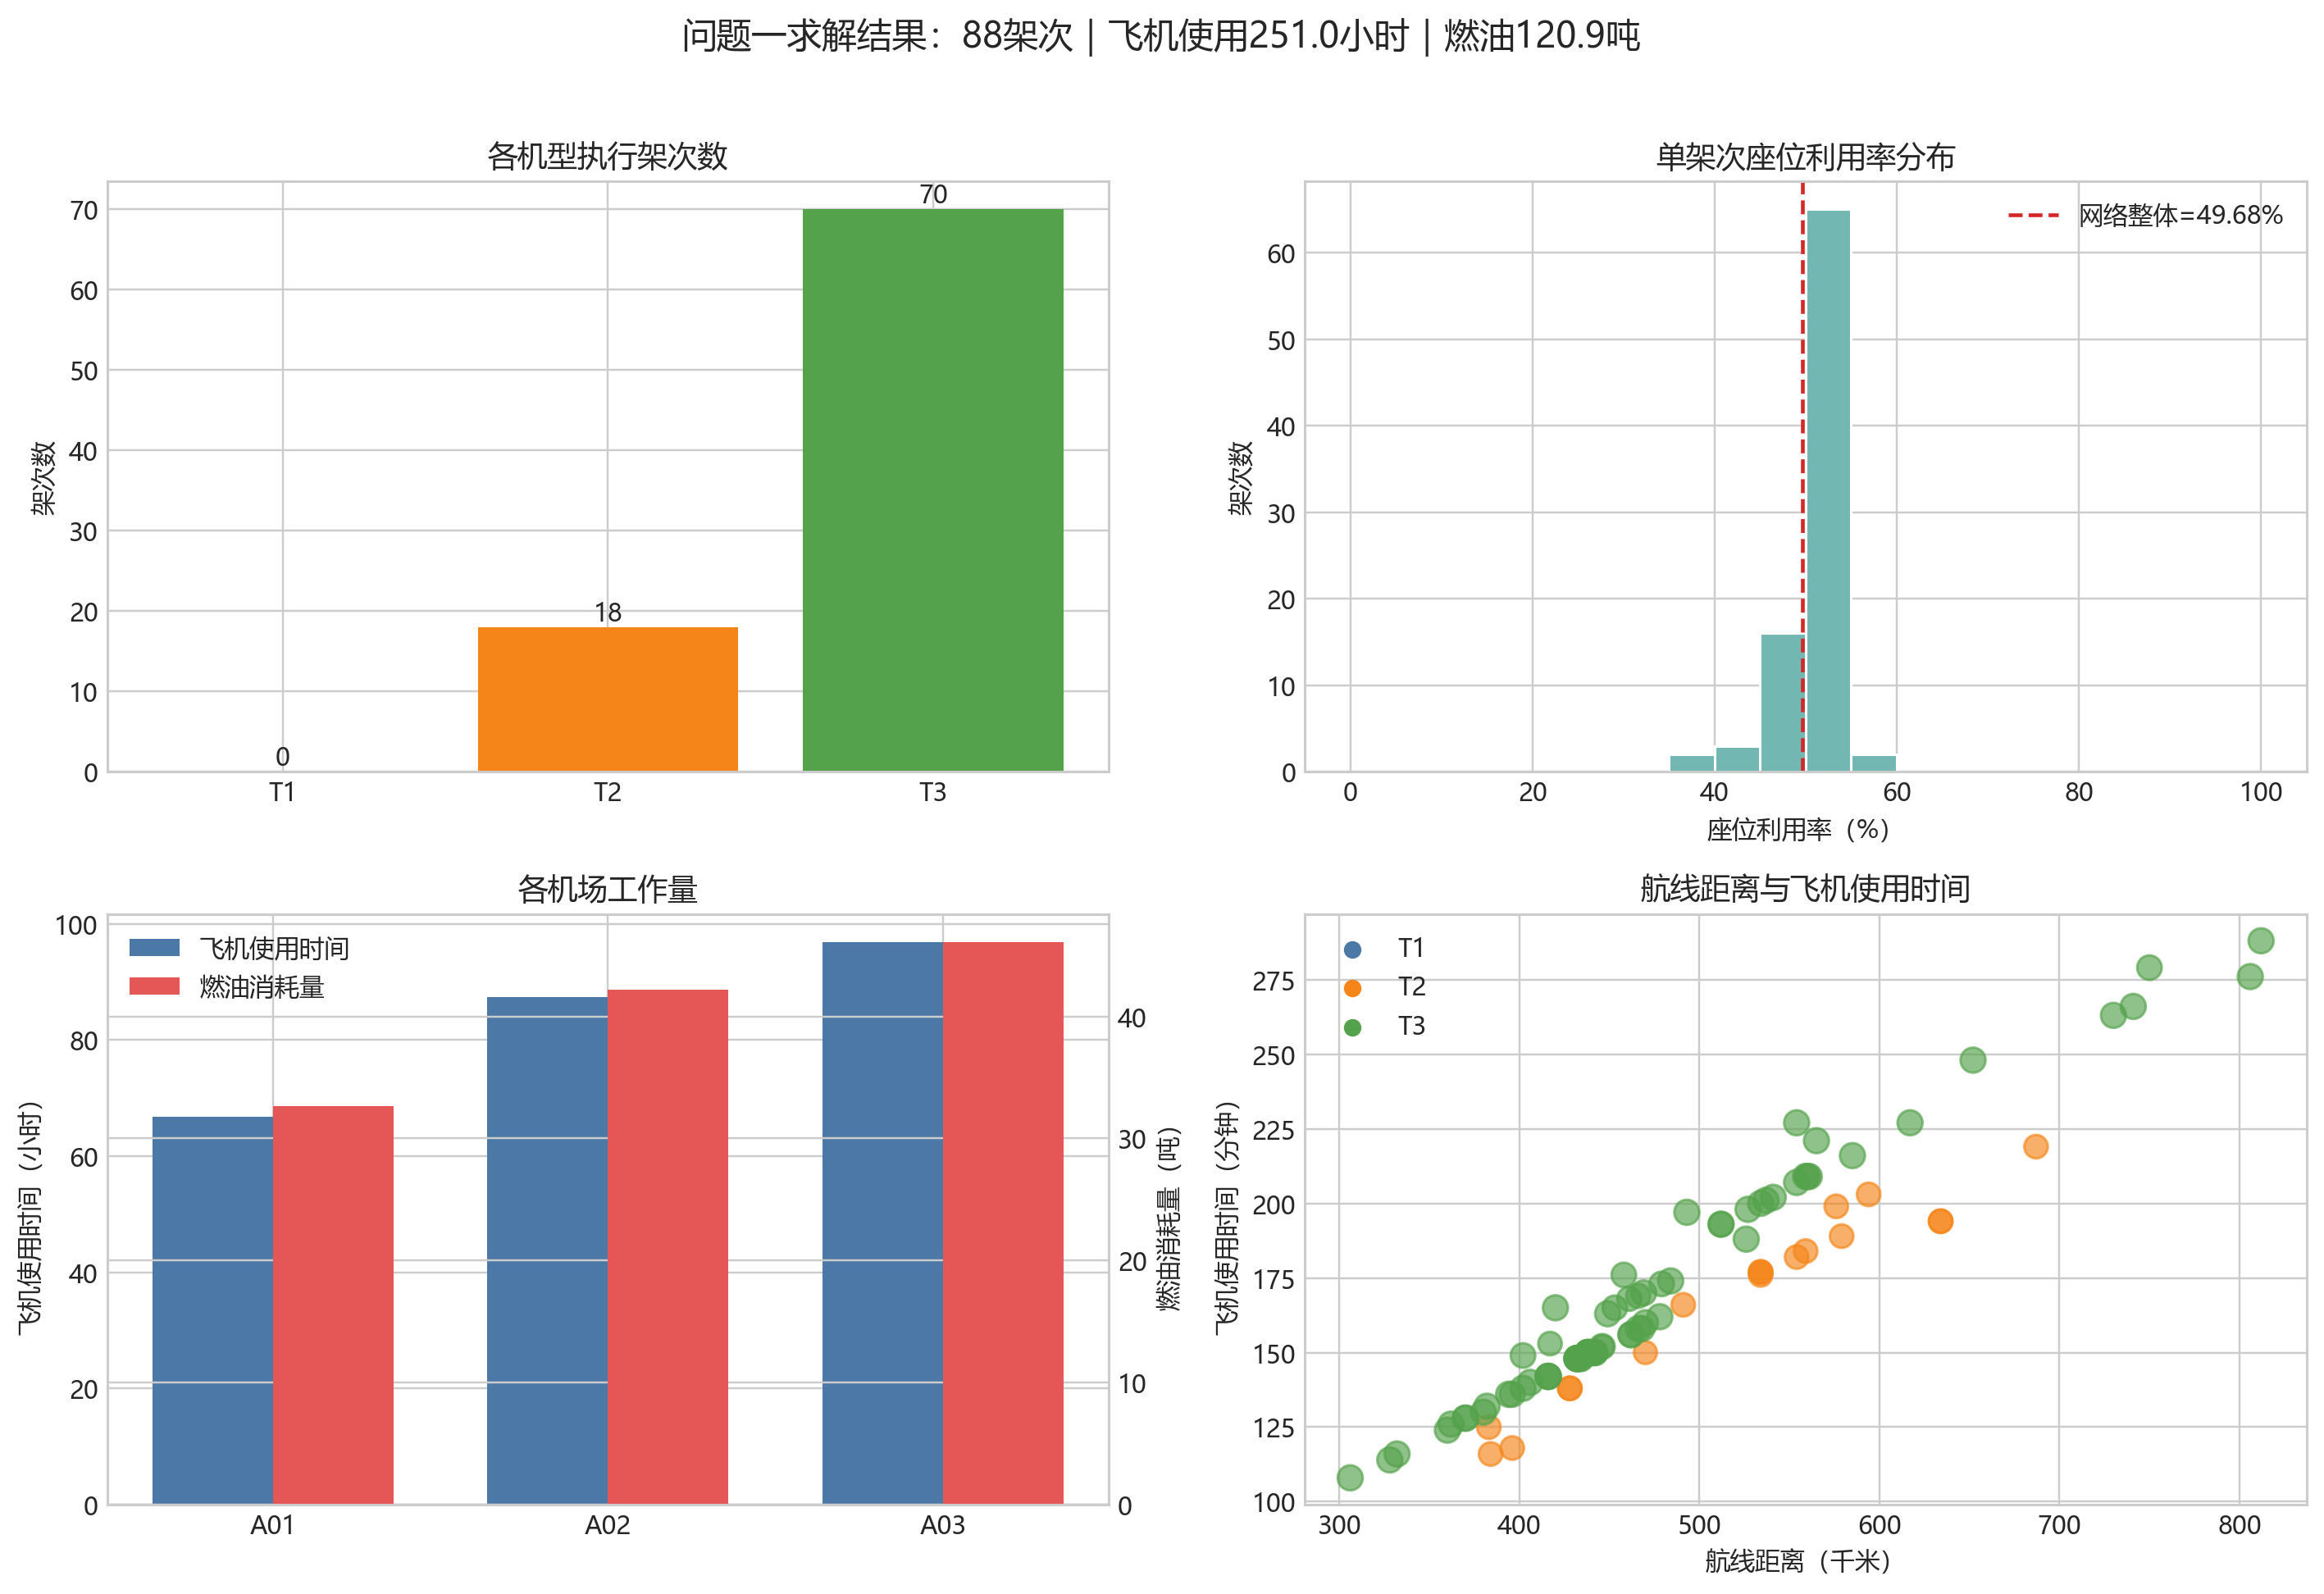
\includegraphics[width=0.95\linewidth]{../output/问题一_求解结果综合图.png}
  \caption{问题一求解结果综合图}
  \label{fig:q1_result}
\end{figure}

\textbf{结果分析}。总飞机使用时间为 15061 分钟（约 251.02 小时），由 88 个架次完成，平均每架次载客约 $1600/88\approx18.2$ 人、使用时间约 171 分钟。座位利用率为 49.68\%（客座公里 $391794.0$ 与可用座公里 $788670.0$ 之比），反映出“满座份满载单飞 + 尾数份合并环游”的拆分策略在缩短总时间与提升利用率之间的折中。求解 gap 仅为 0.13\%（LP 下界 15041.00 分钟），说明所得整数解与理论下界几乎一致，模型与算法接近全局最优。总加油次数为 38 次，对应远端设施（尤其 A03 南端 F037$\sim$F052 段）超航程架次的中途加油需求，与第~\ref{sec:analysis} 节“燃油是硬约束”的判断一致。

\subsection{问题二}

\subsubsection{建模总体思路}

问题二需同时决定出海、海返与穿梭三类人员的运载，整体上是一个带同时取送的车辆路径问题（VRPSPD）。沿用问题一的“解耦 + 分块 + 集合划分”框架：先按设施编号分块固定归属机场（同问题一），将问题解耦为三个结构相同的单机场子问题；再对每个子问题用集合划分建模。与问题一不同的是，问题二以\textbf{OD 对}为覆盖对象（同一 OD 对的人员可互换，按 OD 聚合而非逐人），且\textbf{不再设拆分变量} $y_s$——拆分约束内化到列生成中（枚举只产生“满座 + 一条尾数”的列，等式覆盖自然等价于选机型），主问题更简洁、利于列生成。

\subsubsection{成对拆分与满座往返架次}

沿用问题一“满座 + 尾数”拆分，出海与海返\textbf{成对}进行：设施 $d$ 对机型 $c$ 生成成对尾数 $(d_c,p_c)=(q_d^{\mathrm{out}}\bmod c,\ q_d^{\mathrm{ret}}\bmod c)$，含义是“出海剩 $d_c$ 人、海返剩 $p_c$ 人需合并运送”。满座部分为固定成本：$\lfloor q_d^{\mathrm{out}}/c\rfloor$ 个出海满座 + $\lfloor q_d^{\mathrm{ret}}/c\rfloor$ 个海返满座，因出海$\approx$海返可\textbf{配对为往返满座}（同一架次往返各载 $c$ 人），架次数近半；净残差 $|q_d^{\mathrm{out}}-q_d^{\mathrm{ret}}|\le6$ 极小，基本被尾数吸收。

\subsubsection{候选架次定义与载荷剖面}

尾数合并架次 $r$ 由“机型 $m_r$ + 有向顺序 $S_r=(s_1,\dots,s_k)$ + 每站成对尾数 $(d_t,p_t)$ + 穿梭尾数 $\{h_{(i,j)}\}$”确定。设第 $t$ 站下机 $d_t$ 人（出海到达）、上机 $p_t$ 人（海返出发），穿梭在对应两站之间上下，则逐弧载荷为
\begin{equation}
  L_0=\sum_{t=1}^{k}d_t,\qquad
  L_t=\sum_{u>t} d_u+\sum_{u\le t} p_u+\sum_{i\le t<j} h_{(s_i,s_j)}\quad(t=1,\dots,k),
\end{equation}
其中 $h_{(s_i,s_j)}$ 为本架次自 $s_i$ 穿梭至 $s_j$ 的尾数（$i<j$），其占用 $s_i$ 到 $s_j$ 之间每一弧段上的座位。架次 $r$ 须满足：\textbf{容量} $\max_{0\le t\le k}L_t\le c_{m_r}$；\textbf{先后}（穿梭 $i$ 在 $j$ 前被访问）；\textbf{停靠} $k\le5$；\textbf{燃油}（同问题一）。其 OD 覆盖与成本为
\begin{equation}
  n_{r,(a_r,s_t)}=d_t,\quad n_{r,(s_t,a_r)}=p_t,\quad n_{r,(i,j)}=h_{(i,j)},
\end{equation}
\begin{equation}
  T_r=\frac{d_r^{\mathrm{TSP}}}{v_{m_r}}+10k+10g_r.
\end{equation}

\subsubsection{OD 集合划分主问题}

以 OD 对为覆盖对象建立集合划分主问题：
\begin{equation}
  \min \sum_{r\in\Omega} T_r\lambda_r,\label{eq:q2_obj}
\end{equation}
\begin{equation}
  \text{s.t.}\quad \sum_{r\in\Omega} n_{r,(i,j)}\lambda_r=D_{(i,j)},\quad\forall(i,j),\label{eq:q2_cov}
\end{equation}
\begin{equation}
  \lambda_r\in\mathbb{Z}_+,\label{eq:q2_int}
\end{equation}
其中 $\Omega$ 为候选架次（列）全集，$D_{(i,j)}$ 为 OD 对 $(i,j)$ 的需求总人数。

\subsubsection{求解算法：预枚举 + 惰性加列}

列空间规模约 $5.2\times10^6$ 条（三区块合计），枚举本身秒级完成，但一次性把数百万整数变量塞进集合划分 IP 不可承受，故采用\textbf{列生成}——预枚举全部列，但只在主问题中物化“被用到的列”（惰性加列）。流程如下：

\begin{enumerate}
  \item \textbf{预枚举}：复用问题一的 DFS，扩展为成对尾数 + 穿梭，一次性生成全部候选列 $\Omega$（满座列 + 尾数合并列）；
  \item \textbf{初始受限主问题}：取可行子集 $\Omega'\subset\Omega$（全部满座列 + 每设施单尾数列）；
  \item \textbf{求解 LP}：将式~\eqref{eq:q2_obj}--\eqref{eq:q2_int} 中 $\lambda_r$ 放松为 $\lambda_r\ge0$，得对偶价 $\pi_{(i,j)}$；
  \item \textbf{定价（扫描）}：对 $\Omega$ 逐列计算约化成本，取负者加入 $\Omega'$；
  \item \textbf{迭代}：回到第 3 步，直至无负约化成本列（LP 收敛）；
  \item \textbf{整数化}：在 $\Omega'$ 上分支定界求整数解。
\end{enumerate}

列 $r$ 的\textbf{约化成本}为
\begin{equation}
  \bar c_r=T_r-\sum_{(i,j)}n_{r,(i,j)}\pi_{(i,j)}
  =\frac{d_r^{\mathrm{TSP}}}{v_{m_r}}+10k+10g_r-\sum_{t}\big(d_t\pi^{\mathrm{out}}_{s_t}+p_t\pi^{\mathrm{ret}}_{s_t}\big)-\sum_{(i,j)}h_{(i,j)}\pi^{\mathrm{sh}}_{(i,j)},
\end{equation}
其中 $\pi^{\mathrm{out}}_d,\pi^{\mathrm{ret}}_d,\pi^{\mathrm{sh}}_{(i,j)}$ 为出海、海返、穿梭约束的对偶价。定价就是对 $\Omega$ 做一次 $O(|\Omega|)$ 线性扫描，取 $\bar c_r<-\varepsilon$ 的列加入受限主问题（$\varepsilon$ 为容差）；当 $\min_{r\in\Omega}\bar c_r\ge-\varepsilon$ 时算法收敛。

燃油不写入主问题，而在枚举阶段逐列校验/修复（复用问题一的“相邻加油点间距离 $\le\bar{d}_m$”规则）：超航程者就近插入加油点（绕行计入 $d_r^{\mathrm{TSP}}$、停靠 +20 min 占配额），修复后仍不可行则弃列。

\subsubsection{求解结果与分析}

用上述模型与算法求解，得到问题二的完整运载计划，核心指标见表~\ref{tab:q2_result}，航线网络见图~\ref{fig:q2_network}，求解结果综合对比见图~\ref{fig:q2_result}。

\begin{table}[H]
  \centering
  \caption{问题二求解结果指标}
  \label{tab:q2_result}
  \begin{tabular}{lc}
    \toprule
    指标 & 数值 \\
    \midrule
    总飞机使用时间 & XXX min（$\approx$XXX h） \\
    人员总在途时间 & XXX min（$\approx$XXX h） \\
    总架次数 & XXX \\
    总燃油消耗量 & XXX kg \\
    座位利用率 & XX\% \\
    \midrule
    LP 松弛下界 & XXX min \\
    gap & XX\% \\
    \bottomrule
  \end{tabular}
\end{table}

\begin{figure}[H]
  \centering
  % 待补充：
\includegraphics[width=0.95\linewidth]{../output/问题二_航线网络图.png}
  \fbox{\parbox{0.85\linewidth}{\centering 图占位：问题二航线网络图（待补充） \\[2.5cm]}}
  \caption{问题二航线网络图}
  \label{fig:q2_network}
\end{figure}

\begin{figure}[H]
  \centering
  % 待补充：
\includegraphics[width=0.95\linewidth]{../output/问题二_求解结果综合图.png}
  \fbox{\parbox{0.85\linewidth}{\centering 图占位：问题二求解结果综合图（待补充） \\[2.5cm]}}
  \caption{问题二求解结果综合图}
  \label{fig:q2_result}
\end{figure}

\textbf{结果分析}。（待补充：待求解完成后，结合总飞机使用时间、人员总在途时间、总架次数、总燃油消耗量、座位利用率及 gap 展开分析。）

\subsection{问题三}
（问题三的模型建立与求解待后续完成。）

% ---------------- 六、结论 ----------------
\section{结论}

针对问题一（单向出海运输的直升机运载计划编排），本文将 1600 条出海需求抽象为多机场、多机型、带容量与燃油约束的单向车辆路径问题，利用“人员不可换乘、架次不跨机场、飞机数量充足”三条结构性事实，将问题按机场解耦为三个结构相同的单机场子问题；进一步依据设施沿海岸线的编号分块，把 1353 名 LAND 乘客的机场选择退化为固定参数。在此基础上提出“机型感知拆分 + 集合划分”的精确模型：满座份满载单飞、尾数份跨设施合并为环游，燃油约束简化为“相邻加油点间累计距离不超过最大不加油航程”的可行性判据，并采用“显式枚举候选 + 集合划分整数规划”精确求解。

求解得到：总飞机使用时间 15061 分钟、人员总在途时间 131033 分钟、总架次数 88、总燃油消耗量 120920.1 kg、座位利用率 49.68\%，与 LP 松弛下界的 gap 仅为 0.13\%，说明所得计划接近全局最优。本文方法在保证精确性的同时保持了模型的可解释性，其“解耦 + 分块 + 集合划分”的框架可直接推广至问题二的联合运输与问题三的多日排班场景。

针对问题二（出海、海返与穿梭联合运输），本文将其抽象为带同时取送的车辆路径问题（VRPSPD）：机上人数沿环游先降后升、环游方向成为决策变量。利用“出海与海返逐设施近乎配对、穿梭全部同区块短途”的数据特征，提出“成对拆分、往返环游、穿梭顺路承载”的建模思路，以 OD 对为覆盖对象建立集合划分主问题，并采用“预枚举 + 惰性加列”的列生成算法求解。

求解得到：总飞机使用时间 XXX 分钟、人员总在途时间 XXX 分钟、总架次数 XXX、总燃油消耗量 XXX kg、座位利用率 XX\%，与 LP 松弛下界的 gap 为 XX\%。……（各项数值与结果分析待求解完成后补充。）

% ============================================================
%  AI 工具使用声明（按格式规范要求，置于参考文献之前，二者择一）
% ============================================================
\section*{AI 工具使用声明}

% 未使用 AI 工具时，声明如下：
本参赛队在竞赛过程中未使用任何 AI 工具。

% 使用 AI 工具时，改为下面这条（并删除上一条）：
% 本参赛队在竞赛过程中使用了 AI 工具，主要用于【简要用途，如语言润色、代码调试等】，
% 详细使用情况见支撑材料。

% ============================================================
%  参考文献（二级标题，不编号）
%  引用他人或公开资料的成果必须在此列出，并在正文引用处标注
% ============================================================
\begin{thebibliography}{99}

  \bibitem{ref1} 作者一, 作者二. 论文题目[J]. 期刊名, 年, 卷(期): 起始页--结束页.
  \bibitem{ref2} 作者. 书名[M]. 出版地: 出版社, 出版年.
  \bibitem{ref3} 作者. 网页/文档标题[EB/OL]. 网址, 访问日期.

\end{thebibliography}

% ============================================================
%  附录（二级标题，不编号；页数不限）
%  附录应包括：支撑材料文件列表、全部完整可运行的源程序代码、
%              AI 工具使用声明等
% ============================================================
\section*{附录}

\subsection*{附录 A：支撑材料文件列表}
（列出随论文提交的支撑材料文件名与用途，例如：）
\begin{itemize}
  \item \texttt{code/q1\_solver.py}：问题一求解程序；
  \item \texttt{code/q2\_solver.py}：问题二求解程序；
  \item \texttt{code/q3\_solver.py}：问题三求解程序；
  \item \texttt{AI 工具使用详情.pdf}：AI 工具使用详情说明（如使用 AI 工具）。
\end{itemize}

\subsection*{附录 B：源程序代码}
（贴入建模用到的全部完整、可运行的源程序代码，可直接用 \verb|\lstinputlisting| 引入文件：）
% \lstinputlisting[language=Python]{../code/q1_solver.py}

% 或直接内联粘贴：
% \begin{lstlisting}[language=Python]
% # 在此粘贴源代码
% \end{lstlisting}

\subsection*{附录 C：AI 工具使用声明}
（此处与正文“AI 工具使用声明”一致；如使用 AI 工具，还应说明使用详情，
详见支撑材料中的“AI 工具使用详情.pdf”。）

\end{document}
